\section{\K 滤波电路}
\Par 由于滤波电路的内容比较简单,我们这里就只以桥式滤波电路为例.如图\ref{fig:电桥滤波电路}所示,刚接上电源的时候,电容和负载$R_L$两端接正向整流电压,电容处于充电状态.

\begin{figure}[htbp]
	\centering
	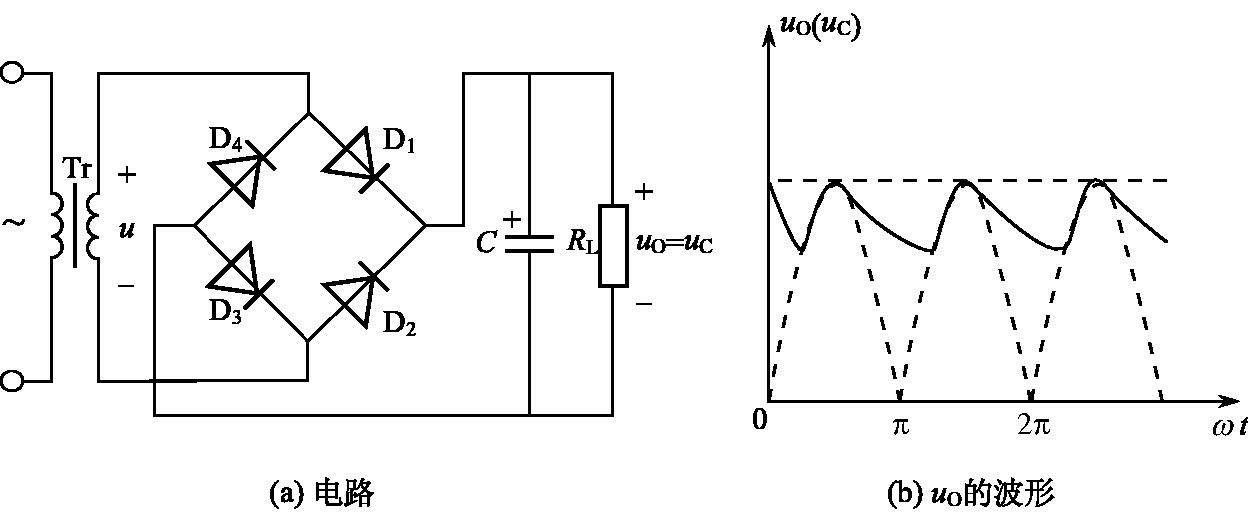
\includegraphics[width=0.55\textwidth]{电桥滤波电路.jpg}
	\caption{电桥滤波电路}
	\label{fig:电桥滤波电路}
\end{figure}

\Par 当电压达到峰值开始下降的时候,电容开始放电.由于电容的放电满足暂态过程,呈指数减小,而整流电压减小的更快,因此电容会维持着$R_L$两端电压让它的减小放缓.

\Par 直到整流电压升高到与电容电压相等,并进一步上升时,电容又开始充电,由此构成了一个循环.

\Par 由上面的分析我们可以知道,电容放电的暂态过程越慢,对我们滤波越有利,因此我们应当选择时间常数$\tau =R_LC$大的电容,通常我们要求
\begin{equation}
    \tau =R_LC\ge 3\sim 5\left( \frac{T}{2} \right) 
\end{equation}